\textbf{\subsection{Расчет  каскада предварительного усиления}}
  \vspace{1em}
  
  Каскад предварительного усиления обеспечивает усиление входного сигнала до необходимого уровня для действия усилителя мощности. Также он выполняет функцию промежуточного звена между регулятором усиления и регулятором тембра.\par

  \begin{figure}[!htbp]
    \center{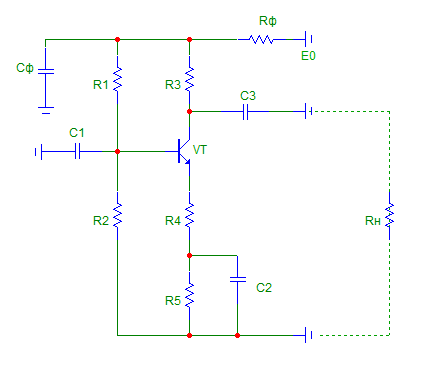
\includegraphics[width=0.6\linewidth]{picture_pre}}
    \caption{Схема каскада предварительного усиления}
    \label{figure:p3_5}
  \end{figure}


  В нашем случае Uн и R н являются входными параметрами регулятора тембра. При двуполярном питании оконечного каскада в качестве источника Ео может использоваться любая из половинок.

  \subsubsection{Амплитуда напряжения и тока нагрузки:}

  \begin{equation}
  \label{eq:equation6_1}
    U_{\text{нм}} = U_{\text{н}} \cdot \sqrt{2} = 0.058 \cdot \sqrt{2} =  0.082~\text{В}
  \end{equation}

  \begin{equation}
  \label{eq:equation6_2}
    I_{\text{нм}} = U_{\text{нм}} / R_{\text{н}} = 0.082 / 4429 = 18.6~\text{мкА}.
  \end{equation}  

  \subsubsection{Ток покоя:}  

  При дальнейшем расчете параметров выбора транзистора необходимо учесть тот факт, что нагрузка подключена в коллекторную цепь. Но по той причине, что ток коллектора будет равен току эмиттера, пренебрегая базовым, в обозначении сразу указан ток коллектора.\par

  \begin{equation}
  \label{eq:equation6_3}
     I_{\text{ок}} \geq (5 \ldots 10) \cdot I_{\text{нм}} = 10 \cdot 18.61 = 186~\text{мкА}.
  \end{equation} 

  Который не удовлетворяет условию тока, необходимому для раскачки УМ: $I_{\text{ок}} = 0.5 \ldots 2$мА. 
  Выбираем ток покоя $I_{\text{ок}}$ = 0.5 мА.


  \subsubsection{Напряжение коллектор-эмиттер транзистора:}  

  \begin{equation}
  \label{eq:equation6_4}
   U_{\text{кэ}} \geq U_{\text{Нm}} + U_{\text{КЭmin}} = 0.058+2 = 2.058~\text{В}.
  \end{equation}   

  При этом $U_{\text{КЭmin}} = 1 \ldots 2$ В.
  Амлитуда сигнала мала, поэтому выбираем $U_{\text{КЭ}} = 4 $В.

  \subsubsection{Напряжение источника питания:}  

  \begin{equation}
  \label{eq:equation6_5}
    E_{\text{0П}} \geq (2 \ldots 3) U_{\text{КЭ}} = 3 \cdot 2 = 6~\text{В};
  \end{equation} 

  \begin{equation}
  \label{eq:equation6_6}
    E_{\text{0}} = (1.2 \ldots 1.3) E_{\text{0П}} = 1.2 \cdot 6 = 7.4~\text{В}.
  \end{equation} 

  \subsubsection{Сопротивление в цепи эмиттера:}  
  
  \begin{equation}
  \label{eq:equation6_7}
    R_{\text{Э}} = R_4 + R_5 = \dfrac{U_{\text{Э}}}{I_{\text{0Э}}} = 0.3 \cdot \dfrac{E_{\text{0П}}}{I_{\text{0К}}}=0.3 \cdot 6.1748 / 0.0002 = 9.95~\text{кОм}.
  \end{equation}

  \subsubsection{Определяем сопротивление R3:} % (fold)

  \begin{equation}
  \label{eq:equation6_8}
     R_3 = \dfrac{ E_{\text{0П}} - U_{\text{КЭ}} - U_{\text{Э}}}{I_{\text{0К}}} = \dfrac{6- 2 -3.6}{0.0002 } = 2775.9~\text{кОм}.
  \end{equation}

  % subsubsection определяем_сопротивление_r3_ (end)
  \subsubsection{Амплитуда тока:} % (fold)
  
  \begin{equation}
  \label{eq:equation6_9}
   I_{\text{Кm}} = \dfrac{U_{\text{нм}}}{R_3} = \dfrac{0.058}{2775.9} = 0.021~\text{мА}
  \end{equation}
  % subsubsection _амплитуда_тока_ (end)
  
  \subsubsection{Мощность, рассеиваемая на коллекторном переходе:} % (fold)

  \begin{equation}
  \label{eq:equation6_10}
    P_{\text{К}} = U_{\text{кэ}} \cdot I_{\text{0К}} = 4 \cdot 0.5 \cdot 10^{-3} = 2~\text{мВт}. 
  \end{equation}
  
  % subsubsection мощность_рассеиваемая_на_коллекторном_переходе_ (end)

  \subsubsection{Критерии выбора транзистора:} % (fold)

  \begin{equation}
  \label{eq:equation6_11}
    P_{\text{К доп}} \geq (1.1 \ldots 1.3) P_{\text{К}} = 1.3 \cdot 2 \cdot 10^{-3} = 2.6~\text{мВт};
  \end{equation} 

  \begin{equation}
   \label{eq:equation6_12}
     U_{\text{КЭ}} \geq E_0 = 12~\text{В};
  \end{equation} 

  \begin{equation}
  \label{eq:equation6_13}
    I_{\text{К доп}} \geq (1.1 \ldots 1.3)(I_{\text{0К}} + I_{\text{Кm}}) = 1.3 \cdot (0.5 \cdot 10^{-3} + 0.0078 \cdot 10^{-3}) = 0.66~\text{мА}; 
  \end{equation} 

  \begin{equation}
   \label{eq:equation6_14}
     f_{h_{21}} \geq (20 \ldots 30) f_{\text{в}} = 30 \cdot 14000 = 420~\text{кГц}
  \end{equation} 
  % subsubsection критерии_выбора_транзистора_ (end)

Расчетный параметр h21:
\begin{equation}
   \label{eq:equation6_15}
h_{21}=\sqrt{h_{21min} \cdot h_{21max}}=\sqrt{40 \cdot 200}=89
\end{equation} 

 \subsubsection{Расчет базвой цепи:}
ток делителя:
 \begin{equation}
   \label{eq:equation6_16}
 I_{\text{Д}}=(5 \ldots 10) \cdot I_{\text{Бm}}=\dfrac{(5 \ldots 10) \cdot I{\text{Кm}}}{h_21}=10 \cdot 7.8\cdot 10^-6 /89=0.87~\text{мкА}
 \end{equation}

 определение сопротивлений базового делителя:
 \begin{equation}
   \label{eq:equation6_17}
   R_1=\dfrac{E_0-U{\text{Э}}-U_{\text{БЭ}}}{I_{\text{ОБ}}+I_{\text{Д}}}=\dfrac{E_0-U_{\text{Э}}-U_{\text{БЭ}}}{ \dfrac{I_{\text{ОК}}}{ h_{21}}+I_{\text{Д}} }
   \end{equation}
   \begin{equation*}
   R_1=(12.3-3.6-0.7)/(0.5 \cdot 10^-3/89+0.87 \cdot 10^-6)=1.2~\text{МОм}
   \end{equation*}

 \begin{equation}
   \label{eq:equation6_18}
   R_2=\dfrac{U_{\text{БЭ}}+U_{\text{Э}}}{I_{\text{Д}}}=(0.7+3.6)/0.87 \cdot 10^-6=5~\text{МОм}
 \end{equation}
\subsubsection{Коэффициент усиления эмиттерного повторителя стремится к 1:}
\begin{equation}
   \label{eq:equation6_19}
K=\dfrac{1+h_21 \cdot R_{\text{ЭН}}}{(1+h_21)\cdot R_{\text{ЭН}}+h_11}=\dfrac{R_{\text{ЭН}}}{R_{\text{ЭН}}+{r_{\text{Э}}}}=2800/(2800+50)=0.0980 \approx 1
\end{equation}
\begin{equation}
   \label{eq:equation6_20}
   r_{\text{Э}}=\dfrac{\psi}{I_0}=25/0.5=50
\end{equation}
\subsubsection{Номинальное входное напряжение:}
\begin{equation}
   \label{eq:equation6_21}
U_{\text{ВХ}}=\dfrac {U_{\text{Н}}}{K}=16 \cdot 10^{-3} /0.98= 16.3~\text {мВ}
\end{equation}
\subsubsection{Входное сопротивление каскада:}
\begin{equation}
   \label{eq:equation6_22}
R_{\text{ВХ}}=\dfrac{1}{\dfrac{1}{R_\text{ВХ Т}}+\dfrac{1}{R_1}+\dfrac{1}{R_2}}=1/(1/256 \cdot 10^3 +1/1.2 \cdot 10^6 + 1/5 \cdot 10^6)=0.2\text{МОм}
\end{equation}
\begin{equation}
   \label{eq:equation6_23}
R_{\text{ВХ Т}}=h_{11}+(1+h_{21})\cdot R_{\text{ЭН}}=h_{21} \cdot h_{\text{Э}}+(1+h_{21}) \cdot R_{\text{ЭН}}=h_{11}+(1+h_{21}) \cdot R_{\text{ЭН}}
\end{equation}
\begin{equation*}
R_{\text{ВХ Т}}=89 \cdot 50+90 \cdot 2800 =256~\text{кОм}
\end{equation*}

\subsubsection{Итоговые данные каскада предварительного усиления:}


\begin{table}[htbp]
\caption{Параметры выбора транзисторов }
\begin{center}\begin{tabular}{|c|c|c|c|c|c|c|}
\hline 
  & тип & $P_{\text{к}}$ доп, мВт & $I_{\text{к}}$ доп, мА & $U_{\text{к}}$ доп, В & $h_{21}$ &  $f_{h_{21}}$, кГц \\ 
\hline 
VT1  & n-p-n & 0.50  & 0.27 & 7.41 & 60 & 540.00\\ 
\hline 
\end{tabular} 
\end{center}
\end{table}

\begin{table}[htbp]
\caption{Режимы работы транзисторов}
\begin{center}\begin{tabular}{|c|c|c|c|c|c|c|c|c|c|c|c|c|}
\hline 
   & $I_\text{0К}$ & $I_\text{0б}$& $U_\text{0Б}$ & $U_\text{0К}$&  $I_{\text{Км}}$  & $I_{\text{Бм}}$& $U_{\text{км}}$, B & $P_{\text{к}}$ & K\\ 
  & мА & мА& В & В & мА & мА & B & мВт & \\
\hline 
КТ127А-1 & 1 & 0.03 & 0.7 & 5 & 50 & 1.66 & 25 & 15 & 0.99 \\
\hline 
КТ127Б-1 & 1  &  0.01  &  0.6  & 5  & 20 &   0.22  &  20  &  15  &  13  &  0.98 \\
\hline
\end{tabular} 
\end{center}
\end{table}

